\chapter{Experimental setup}
In this chapter we describe the setup we use for our experiments. Our most prominent contribution is the proposal of a tool called CloneRefactor. This tool allows us to map clones with all clone definitions as described in chapter \ref{chap:clonetypes}.

All results of our experiments, as displayed in chapter \ref{ch:results}, are measured over a corpus of Java projects. In this chapter we will explain how we prepared this corpus.

\section{The corpus}\label{chap:corpus}
For our measurements we use a large corpus of open source projects \cite{githubCorpus2013}. This corpus has been assembled to contain relatively higher quality projects. Also, any duplicate projects were removed from this corpus. This results in a variety of Java projects that reflect the quality of average open source Java systems and are useful to perform measurements on.

As indicated in chapter \ref{chap:challenge} CloneRefactor requires all libraries of software projects we test. As these are not included in the used corpus \cite{githubCorpus2013}, we decided to filter the corpus to only include Maven projects. Maven is a build automation tool used primarily for Java, and works on basis of an \texttt{pom.xml} file to describe the projects' dependencies. As no \texttt{pom.xml} files are included in the corpus, we cloned the latest version of each project in the corpus. We then removed each project that has no \texttt{pom.xml} file. As a final step, we collected all dependencies for each project by using the \texttt{mvn dependency:copy-dependencies -DoutputDirectory=lib} Maven command, and removed each project for which not all dependencies were available (due to non-Maven dependencies being used or unsatisfiable dependencies being referenced in the \texttt{pom.xml} file).

Some general data regarding this corpus is displayed in Table \ref{table:general}.

\begin{table}[H]
  \begin{center}
  \caption{General results for GitHub Java projects corpus \cite{githubCorpus2013}.} \label{table:general}
  \medskip
\begin{tabular}{|l|l|}
\hline
Amount of projects                                                                                      & 1,361      \\ \hline
\begin{tabular}[c]{@{}l@{}}Amount of lines (excluding\\whitespace, comments and newlines.)\end{tabular} & 1,414,996  \\ \hline
Amount of statements/declarations                                                                       & 1,212,189  \\ \hline
\begin{tabular}[c]{@{}l@{}}Amount of tokens (excluding\\whitespace, comments and newlines.)\end{tabular} & 11,643,194 \\ \hline
\end{tabular}
\end{center}
\end{table}

\chapter{Results}

\label{ch:results}
In this chapter, we present the results of our experiments.

\section{Thresholds} \label{sec:thresholds}

\section{Relation, Location and Content Analysis of Clones}\label{chap:clonecontextexpl}
To be able to refactor code clones, it is very important to consider the context of the clone. We define the following aspects of the clone as its context:
\begin{enumerate}
  \item The relation of clone instances among each other through inheritance (for example: a clone instance resides in a superclass of another clone instance in the same clone class).
  \item Where a clone instance occurs in the code (for example: a method-level clone is a clone instance that is in a method).
  \item The contents of a clone instance (for example: the clone instance spans several methods).
\end{enumerate}

\begin{figure}[H]
  \caption{Abstract representation of clone classes and clone instances.}
    \medskip
    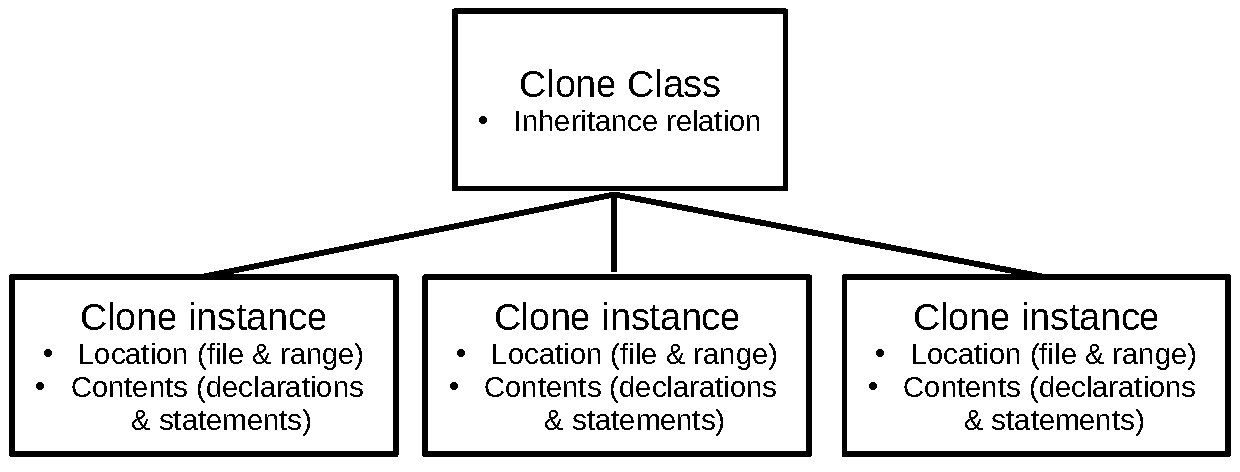
\includegraphics[width=1\columnwidth]{img/context}
  \label{fig:clonecontext}
\end{figure}

Figure \ref{fig:clonecontext} shows an abstract representation of clone classes and clone instances. The relation of clones through inheritance is measured on clone class level: it involves all child clone instances. The location and contents of clones is measured on clone instance level. A clone's location involves the file it resides in and the range it spans (for example: line 6 col 2 - line 7 col 50). A clone instance contents consists of a list of all statements and declarations it spans.

We analyzed the context of clones in a large corpus of open source projects. For these experiments, we used our CloneRefactor tool. These experiments follow the structure of the context: The relation between clone instances is explained, measured and discussed in chapter \ref{chap:relationsinstances}; the location of clone instances is explained, measured and discussed in chapter \ref{chap:clonelocation};  the content of clone instances are explained, measured and discussed in chapter \ref{chap:clonecontents}.

\subsection{Clone detection results}
Currently, we have implemented two clone detection algorithms into CloneRefactor. The first one finds clones by comparing tokens (excluding whitespace, comments and newlines), equal to the definition of type 1 clones in literature \cite{roy2007survey}. The second algorithm implements our type 1R, as explained in chapter \ref{chap:type1clones}. The differences between the clones found for these algorithms is displayed in Table \ref{table:clonedet}.

\begin{table}[H]
  \begin{center}
  \caption{CloneRefactor clone detection results for the two different algorithms.} \label{table:clonedet}
  \medskip
\begin{tabular}{|l|l|l|}
\hline
 & \textbf{Type 1} & \textbf{Type 1R} \\ \hline
\begin{tabular}[c]{@{}l@{}}Amount of lines cloned\end{tabular} & 200,362 & 129,519 \\ \hline
\begin{tabular}[c]{@{}l@{}}Amount of statements/\\declarations cloned\end{tabular} & 182,466 & 118,980 \\ \hline
\begin{tabular}[c]{@{}l@{}}Amount of tokens cloned\end{tabular} & 1,582,845 & 973,596 \\ \hline
\end{tabular}
\end{center}
\end{table}

Looking at Table \ref{table:clonedet}, it becomes apparent that the type 1R algorithm finds significantly less clones than the type 1 algorithm. This indicates that about a third of the clones have textual equality, but are not actually equal when considering the types of expressions. This makes these clones less suitable for automated refactoring.

\subsection{Relations Between Clone Instances} \label{chap:relationsinstances}
When merging code clones in object-oriented languages, it is very important to consider the relation between clone instances. This relation has a big impact on how a clone should be merged, in order to improve the software design in the process. In this chapter, we display measurements we conducted on the corpus introduced in chapter \ref{chap:corpus}. These measurements are based on an experiment by Fontana et al. \cite{fontana2015duplicated}, which we will briefly introduce in chapter \ref{chap:catcloneinstancerelations}. We use a vastly different setup, which is explained in chapter \ref{chap:oursetup}. We then show our results in chapter \ref{chap:ourmeasurements}.

\subsubsection{Categorizing Clone Instance Relations}\label{chap:catcloneinstancerelations}
Fontana et al. \cite{fontana2015duplicated} describe measurements on 50 open source projects on the relation of clone instances to each other. To do this, they first define several categories for the relation between clone instances in object-oriented languages. A few of these categories are shown in Figure \ref{fig:clonerelation}. These categories are as follows:
\begin{enumerate}
  \item \textbf{Same method}: All instances of the clone class are in the same method.
  \item \textbf{Same class}: All instances of the clone class are in the same class.
  \item \textbf{Superclass}: All instances of the clone class are children and parents of each other.
  \item \textbf{Ancestor class}: All instances of the clone class are superclasses except for the direct superclass.
  \item \textbf{Sibling class}: All instances of the clone class have the same parent class.
  \item \textbf{First cousin class}: All instances of the clone class have the same grandparent class.
\item \textbf{Common hierarchy class}: All instances of the clone class belong to the same hierarchy, but do not belong to any of the other categories.
\item \textbf{Same external superclass}: All instances of the clone class have the same superclass, but this superclass is not included in the project but part of a library.
\item \textbf{Unrelated class}: There is at least one instance in the clone class that is not in the same hierarchy.
\end{enumerate}

\begin{figure}[H]
  \caption{Abstract figure displaying some relations of clone classes. Arrows represent superclass relations.}
    \medskip
    \centering
    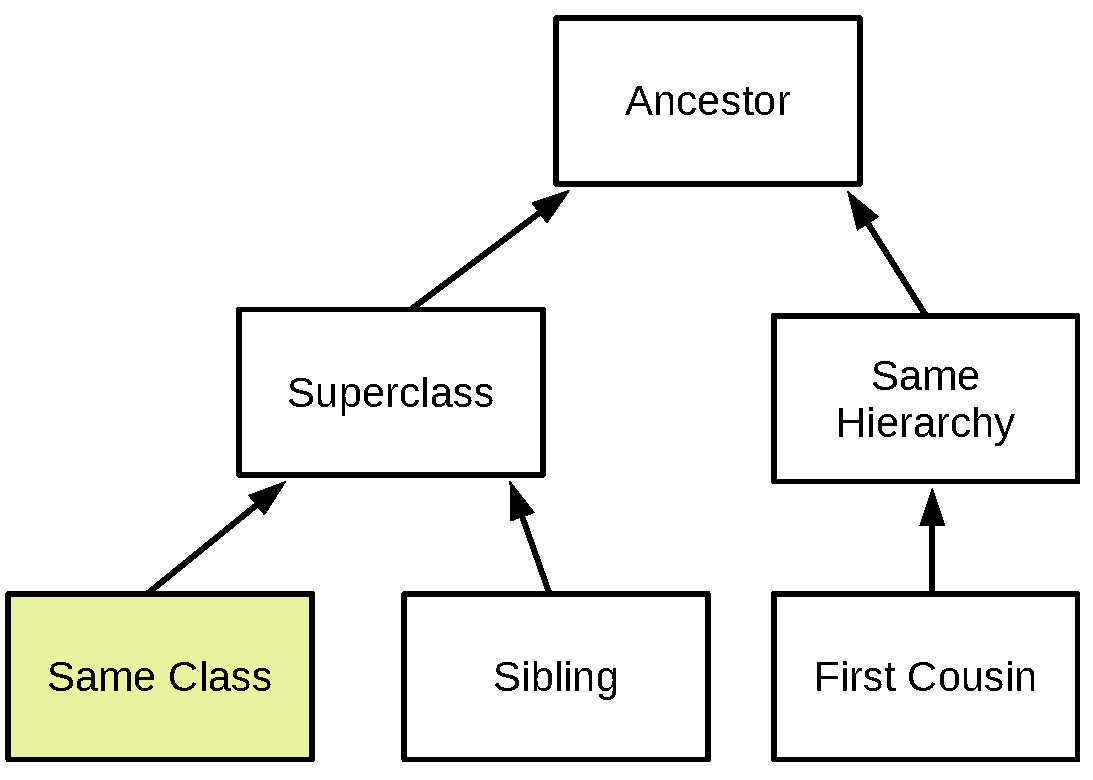
\includegraphics[width=0.6\columnwidth]{img/Relation}
  \label{fig:clonerelation}
\end{figure}
Please note that none of these categories allow external classes (except for ``same external superclass''). So if two clone instances are related through external classes but do not share a common external superclass, it will be flagged as ``unrelated''. The main reason for this is that it is (often) not possible to refactor to external classes.

\subsubsection{Our setup}\label{chap:oursetup}
We use a similar setup to that used by Fontana et al. (Table~3 of Fontana et al. \cite{fontana2015duplicated}). Fontana et al. measure clones using their own tool (DCRA). As explained in chapter~\ref{ch:tool-overview}, we chose to implement our own tool, CloneRefactor. Therefore, the setup for our measurements differs as follows from Fontana et al.:
\begin{itemize}
  \item We consider clone classes rather than clone pairs. The rationale for this is given in chapter \ref{chap:cloneclasses}.
\item We use different thresholds regarding when a clone should be considered. Fontana et al. seek clones that span a minimum of 7 source lines of code (SLOC). We seek clones with a minimum size of 6 statements/declarations. This is explained detail in chapter \ref{chap:thresholds}.
\item We seek duplicates by statement/declaration rather than SLOC. This makes our analysis depend less on the coding style (in terms of newline usage) of the author of the software project.
\item We test a broader range of projects. Fontana et al. use a set of 50 relatively large projects. We use the corpus as explained in \ref{chap:corpus}, which contains a diverse set of projects (diverse both in volume and code quality).
\end{itemize}

\subsection{Our results} \label{chap:ourmeasurements}
Table~\ref{table:relations} contains our results regarding the relations between clone instances. In this table, ``T1'' stands for the type 1 algorithm from literature and ``1R'' stands for our type 1R definition as explained in chapter \ref{chap:type1clones}.

\begin{table}[H]
  \begin{center}
  \caption{Clone relations} \label{table:relations}
  \medskip
\begin{tabular}{|l|l|l|l|l|} \hline
\textbf{Relation}  & \textbf{\# T1} & \textbf{\% T1}  & \textbf{\# 1R} & \textbf{\% 1R} \\ \hline
Unrelated          & 6,134           & 35.48  & 4,762 & 38.14            \\ \hline
\begin{tabular}[c]{@{}l@{}}Same\\Class\end{tabular}          & 4,772            & 27.60  & 3,131 & 25.07             \\ \hline
Sibling            & 2,680            & 15.50   & 1,949 & 15.61            \\ \hline
\begin{tabular}[c]{@{}l@{}}Same\\Method\end{tabular}         & 2,247            & 13.00   & 1,685 & 13.49             \\ \hline
\begin{tabular}[c]{@{}l@{}}External\\Superclass\end{tabular} & 794            & 4.59   & 558 & 4.47             \\ \hline
\begin{tabular}[c]{@{}l@{}}First\\Cousin\end{tabular}        & 269             & 1.56     & 197 & 1.58           \\ \hline
Superclass         & 237             & 1.37     & 118 & 0.94           \\ \hline
\begin{tabular}[c]{@{}l@{}}Common\\Hierarchy\end{tabular}    & 123             & 0.71    & 73 & 0.58            \\ \hline
Ancestor           & 35              & 0.20     & 14 & 0.11          \\ \hline
\end{tabular}
\end{center}
\end{table}

The most notable difference when comparing it to the results of Fontana et al. \cite{fontana2015duplicated} is that in our results most of the clones are unrelated (38.14\% with type 1R), while for them it was only 15.70\%. This might be due to the fact that we consider clone classes rather than clone pairs, and mark the clone class ``Unrelated'' even if just one of the clone instances is outside a hierarchy. It could also be that the corpus which we use, as it has generally smaller projects, uses more classes from outside the project (which are marked ``Unrelated'' if they do not have a common external superclass). About a fourth of all clone classes have all instances in the same class, which is generally easy to refactor. On the third place come the ``Sibling'' clones, which can often be refactored using a pull-up refactoring. There are no noteworthy differences between type 1 and type 1R clones.

\subsection{Clone instance location}\label{chap:clonelocation}
After mapping the relations between individual clones, we looked at the location of individual clone instances. A paper by Lozano et al. \cite{lozano2007evaluating} discusses the harmfulness of cloning. The authors argue that 98\% are produced at method-level. However, this claim is based on a small dataset and based on human copy-paste behavior rather than static code analysis. We validated this claim over our corpus. The results for the clone instance locations are shown in Table \ref{table:locations}. We chose the following categories:
\begin{enumerate}
  \item \textbf{Method/Constructor Level:} A clone instance that does not exceed the boundaries of a single method or constructor (optionally including the declaration of the method or constructor itself).
  \item \textbf{Class Level:} A clone instance in a class, that exceeds the boundaries of a single method or contains something else in the class (like field declarations, other methods, etc.).
  \item \textbf{Interface Level:} A clone that is (a part of) an interface.
  \item \textbf{Enumeration Level:} A clone that is (a part of) an enumeration.
\end{enumerate}

Please note that these results are measured over each clone instance rather than each clone class, hence the higher total amount in comparison to the results of chapter \ref{chap:ourmeasurements}.

\begin{table}[H]
  \begin{center}
  \caption{Clone instance locations} \label{table:locations}
  \medskip
\begin{tabular}{|l|l|l|l|l|}
\hline
\textbf{Location}  & \textbf{\# T1} & \textbf{\% T1}  & \textbf{\# 1R} & \textbf{\% 1R} \\ \hline
Method Level       & 32,861           & 66.02   & 19,075 & 58.23            \\ \hline
Class Level        & 15,069           & 30.27   & 12,207 & 37.27            \\ \hline
\begin{tabular}[c]{@{}l@{}}Constructor\\Level\end{tabular}  & 1,391            & 2.79     & 1,080 & 3.30           \\ \hline
\begin{tabular}[c]{@{}l@{}}Interface\\Level\end{tabular}    & 282              & 0.57     & 247 & 0.75           \\ \hline
Enum Level         & 171               & 0.34    & 147 & 0.45            \\ \hline
\end{tabular}
\end{center}
\end{table}

Our results indicate that around 58\% of the clones are produced at method-level. About 39\% of clones either span several methods/constructors or contain something like a field declaration. Another 3\% of the clones are found in constructors. The amount of clones found in interfaces and enumerations is very low. Regarding the differences between type 1 and type 1R, it seems that there are relatively less method level clones and more class level clones for type 1R. This is probably due to that the main reason for variability between type 1 and type 1R is variable references, which occur more at method level than class level.

\section{Clone instance contents}\label{chap:clonecontents}
Finally, we looked at the contents of individual clone instances: what kind of declarations and statements do they span. We selected the following categories to be relevant for refactoring:
\begin{enumerate}
  \item \textbf{Full Method/Class/Interface/Enumeration:} A clone that spans a full class, method, constructor, interface or enumeration, including its declaration.
  \item \textbf{Partial Method/Constructor:} A clone that spans a method partially, optionally including its declaration.
  \item \textbf{Several Methods:} A clone that spans over two or more methods, either fully or partially, but does not span anything but methods (so not fields or anything in between).
  \item \textbf{Only Fields:} A clone that spans only global variables.
  \item \textbf{Includes Fields/Constructor:} A clone that spans a combination of fields and other things, like methods.
  \item \textbf{Method/Class/Interface/Enumeration Declaration:} A clone that contains the declaration (usually the first line) of a class, method, interface or enumeration.
  \item \textbf{Other:} Anything that does not match with above-stated categories.
\end{enumerate}

The results for these categories are displayed in Table \ref{table:contents}.

\begin{table}[H]
  \begin{center}
  \caption{Clone instance contents} \label{table:contents}
  \medskip
\begin{tabular}{|l|l|l|l|l|}
  \hline
  \textbf{Contents} & \textbf{\# T1} & \textbf{\% T1}  & \textbf{\# 1R} & \textbf{\% 1R} \\ \hline
  \begin{tabular}[c]{@{}l@{}}Partial\\Method\end{tabular}             & 32,214 & 64.72 & 18,791 & 57.37 \\ \hline
  \begin{tabular}[c]{@{}l@{}}Several\\Methods\end{tabular}            & 10,542 & 21.18 & 8,514 & 25.99 \\ \hline
  \begin{tabular}[c]{@{}l@{}}Includes\\Constructor\end{tabular}       & 1,772  & 3.56  & 1,213 & 3.70 \\ \hline
  Includes Field                                                      & 1,681  & 3.38  & 1,487 & 4.54 \\ \hline
  \begin{tabular}[c]{@{}l@{}}Partial\\Constructor\end{tabular}        & 1,389  & 2.79  & 1,078 & 3.29 \\ \hline
  Only Fields                                                         & 962    & 1.93  & 888 & 2.71 \\ \hline
  Full Method                                                         & 647    & 1.30  & 284 & 0.87 \\ \hline
  \begin{tabular}[c]{@{}l@{}}Includes Class\\Declaration\end{tabular} & 263    & 0.53  & 258 & 0.79 \\ \hline
  \begin{tabular}[c]{@{}l@{}}Other\\Categories\end{tabular}           & 304    & 0.61  & 243 & 0.74 \\ \hline
\end{tabular}
\end{center}
\end{table}

Unsurprisingly, most clones span a part of a method. More than a quarter of the clones (for type 1R) span over several methods, which either requires more advanced refactoring techniques or indicates a non-harmful clone.

\section{Merging duplicate code through refactoring}
The most used technique to merge clones is method extraction (creating a new method on basis of the contents of clones). However, method extraction cannot be applied in all cases. Sometimes a clone spans a statement partially (like a for-loop of which only it's declaration and a part of the body is cloned). Merging the clones can be harder in such instances. Also, the cloned code can contain statements like \texttt{return}, \texttt{break}, \texttt{continue}. In these instances, more conditions may apply to be able to conduct a refactoring, if beneficial at all.

We measured the amount of clones that can be refactored through method extraction (without additional transformations being required). Our results are displayed in Table \ref{table:refactorability}. In this table we use the following categories:
\begin{itemize}
    \item \textbf{Can be extracted:} This clone is a fragment of code that can directly be extracted to a method. Then, based on the relation between the clone instances, further refactoring techniques can be used to merge the extracted methods (for instance ``pull up method'' for clones in sibling classes).
    \item \textbf{Complex control flow:} This clone contains \texttt{break}, \texttt{continue} or \texttt{return} statements.
    \item \textbf{Spans part of a block:} This clone spans a part of a statement.
    \item \textbf{Is not a partial method:} If the clone does not fall in the ``Partial method'' category of Table \ref{table:contents}, the ``extract method'' refactoring technique cannot be applied.
\end{itemize}

\begin{table}[H]
  \begin{center}
  \caption{Refactorability through method extraction} \label{table:refactorability}
  \medskip
\begin{tabular}{|l|l|l|l|l|}
\hline
\textbf{}        & \textbf{\# T1} & \textbf{\% T1}  & \textbf{\# 1R} & \textbf{\% 1R} \\ \hline
\begin{tabular}[c]{@{}l@{}}Is not a\\partial method\end{tabular}           & 5,917 & 34.22 & 4,806 & 38.49 \\ \hline
\begin{tabular}[c]{@{}l@{}}Complex\\control flow\end{tabular} & 5,511 & 31.87 & 3,158 & 25.29 \\ \hline
\begin{tabular}[c]{@{}l@{}}Spans part of\\a block\end{tabular}             & 3,989 & 23.07 & 3,152 & 25.24 \\ \hline
\begin{tabular}[c]{@{}l@{}}Can be\\extracted\end{tabular}                  & 1,874 & 10.84 & 1,371 & 10.98 \\ \hline
\end{tabular}
\end{center}
\end{table}

From Table \ref{table:refactorability}, we can see that approximately ten percent of the clones can directly be refactored through method extraction (and possibly other refactoring techniques based on the relation of the clone instances). For the other clones, other techniques or transformations will be required. Looking into these techniques and transformations will be one of our next steps.
